\documentclass[10pt]{article}
\usepackage{hyperref}
\usepackage[utf8]{vietnam}
\usepackage[margin=1in]{geometry} 
\usepackage{amsmath,amsthm,amssymb, graphicx, multicol, array}
\usepackage{epigraph}
\newcommand{\N}{\mathbb{N}}
\newcommand{\Z}{\mathbb{Z}}
 
\newenvironment{problem}[2][Problem]{\begin{trivlist}
\item[\hskip \labelsep {\bfseries #1}\hskip \labelsep {\bfseries #2.}]}{\end{trivlist}}



\begin{document}
\title{Linear Regression}
\author{Hoang Nguyen, Huy Nguyen}
\maketitle

\epigraph{In God we trust, all others must bring data.}{\textit{W.Edwards Deming}}

\section{Heuristics of the linear regression}
- Linear model đơn giản nhất là một model thể hiện được một tổ hợp tuyến tính   các thành phần của input variables:
\[ y(x,w) = w_0 + w_1x_1 + ... +w_Dx_D \]
Trong đó, $x = (x_1, ...,x_D)^{T}$. Đây được gọi là linear regression. Chìa khóa của mô hình này tính tuyến tính của các tham số $w_0, w_1,..w_D$. Chú ý rằng đối với model này ta cũng có thể xem là tuyến tính với các input variables $x_i$, và đây cũng là điểm yếu vì nếu chỉ dựa vào model này thì ta chỉ có thể xây dựng được một đường thẳng để ước lượng được mối tương quan giữa x và y. Chính vì thế người ta đã mở rộng mô hình bằng cách xem xét thêm tổ hợp tuyến tính của các hàm số phi tuyến tính của input theo biểu thức sau:
\[ y(x, w) = w_0 + \sum_{i=1}^{D}w_i\phi_{i}(x) \]
Trong đó $w=(w_0,...,w_{D})^{T}$ và $\phi=(\phi_1,...,\phi_{D})^{T}$.\\
- Bằng cách sử dụng các hàm phi tuyến tính $\phi$, ta có thể quan sát được rằng $y(x,w)$ trở thành một hàm phi tuyến tính đối với vector input x. Mặc dù vậy, hàm $(x,w)$ vẫn là một hàm tuyến tính đối với w.\\
- Có rất nhiều cách để chọn hàm phi tuyến tính $\phi$ (Hình 1), một ví dụ rất được ứng dụng rộng rãi trong machine learning là:
\[ \phi_{i}=\sigma(\frac{x-\mu}{s}) \]
Trong đó $\sigma(a)$ là hàm sigmoid và được định nghĩa: $\sigma(a) = \frac{1}{1 + e^{-a}}$.\\
Một ví dụ khác xuất hiện nhiều trong signal processing đó là $\phi$ thường được chọn như chuỗi Fourier, dẫn đến sự khai triển của hàm sin. Mình không hiểu rõ về signal processing, xin nhường sự giải thích cho những ai hiểu về signal processing :))
\begin{figure}
  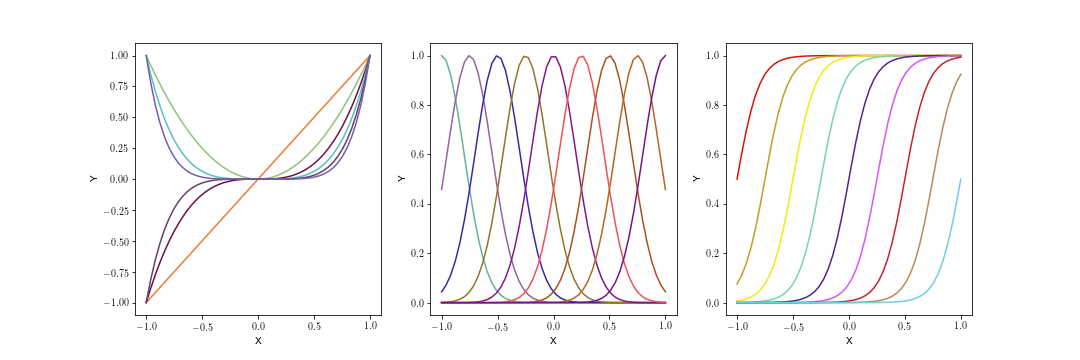
\includegraphics[width=\linewidth]{kernel.png}
  \caption{Một vài ví dụ về hàm phi tuyến tính $\phi$ hay được sử dụng, bên trái ngoài cùng là hàm đa thức, ở giữa là hàm Gausian, và ngoài cùng bên phải là hàm sigmoid}
  \label{fig:boat1}
\end{figure}
\section{Least Squared Error} 
\begin{enumerate}
\item X là số thực.


Giả sử $X \in \mathbb{R}$ và $Y \in \mathbb{R}$ là 2 biến ngẫu nhiên (không nhất thiết phải độc lập) sao cho $\mathbb{V}[X] \neq 0$.
\begin{itemize}

\item Định nghĩa: Theorical linear regression của X trên Y là một xấp xỉ tốt nhất (best approximation) ở dạng bậc hai (in quadratic means) của Y bởi một hàm số tuyến tính của X (ví dụ $a + bX$), trong đó a và b là 2 số thực sao sao cho $\mathbb{E}[(Y - a - bX)^2]$ đạt giá trị nhỏ nhất.
\end{itemize}

Dựa vào định nghĩa trên ta xây dựng một hàm số $f:(a,b)\longmapsto \mathbb{E}[(Y - a - bX)^2$. Ta có thể xem $f$ là một hàm số của a và b "đo" độ gần của điểm (X,Y) với đường thẳng $y = a + bx$ ở kỳ vọng (in expectation). Lấy đạo hàm $f$ theo a, b và set bằng 0, ta có:
\[\begin{cases} \frac{\partial f}{\partial \tilde{a}} = 0 \\ \frac{\partial f}{\partial 0} = 0\end{cases} \Longleftrightarrow \begin{cases} \mathbb{E}[Y-(a+bX)] =0 \\ \mathbb{E}\Big[X \Big(Y-(a+bX) \Big)\Big] =0 \end{cases} \Longleftrightarrow \begin{cases}  \mathbb{E}[Y] = a + b\mathbb{E}[X] \tag{1} \\ \mathbb{E}[XY] =  a\mathbb{E}[X] + b\mathbb{E}[X^2]  \end{cases}  \] 
\[\Longleftrightarrow  \mathbb{E}[XY] = \mathbb{E}[X]\mathbb{E}[Y] - b(\mathbb{E}[X])^2 + b\mathbb{E}[X^2] \Longleftrightarrow b(\mathbb{E}[X])^2 - b\mathbb{E}[X^2] = \mathbb{E}[X]\mathbb{E}[Y] \Longleftrightarrow b= \frac{Cov(X,y)}{Var(X)}\]
Thay b vào biểu thức: $\mathbb{E}[Y] = a + b\mathbb{E}[X]$, ta có $a=\mathbb{E}[Y] - \frac{Cov(X,Y)}{Var(X)}\mathbb{E}[X]$.\\
Đặt $\epsilon = Y - (a+bX)$, ta có được: $Y = a + bX + \epsilon $ với $\mathbb{E}[\epsilon] = 0$ và $Cov(X, \epsilon) = 0$(suy ra từ (1)). Giả sử ngược lại, nếu ta có điểm $(X, Y)$ và đường thẳng $y = ax + b$ nào đó thỏa mãn:\\
\begin{itemize}
\item $Y = a+bX+\epsilon$ với $a,b \in \mathbb{R}$ 
\item $\epsilon$ là một random variable thỏa mãn $Cov(X,\epsilon) = 0$ và $\mathbb{E}[\epsilon] = 0$

\end{itemize}
Thì $a+bX$ là một theoretical linear regression của Y trên X.\\ 
Giả sử ta có một tập hợp i.i.d các điểm $(X_1, Y_1),...(X_n, Y_n)$ theo phân phối như sau: $Y_i = a + bX_i + \epsilon$ (thỏa mã các điều kiện trên).
\begin{itemize}

\item Định nghĩa: Ước lượng Least Squared Error (LSE) của (a,b) là $(\hat{a}, \hat{b})$ sao cho tổng bình phương sai số sau là nhỏ nhất:
\[ \sum_{i=1}^{n} (Y_i - a - bX_i)^2 \]

\end{itemize}

Lưu ý rằng dựa vào chứng minh phía trên ta có $a=\mathbb{E}[Y] - \frac{Cov(X,Y)}{Var(X)}\mathbb{E}[X]$ và $b= \frac{Cov(X,y)}{Var(X)}$ là các giá trị làm tổng bình phương sai số là nhỏ nhất. Mục tiêu của ta là tìm $(\hat{a}, \hat{b})$ càng tiệm cận (a,b) càng tốt. Vì vậy, dựa vào law of large number được phát phiểu như sau:
\[ \bar{X_n} \xrightarrow[n \longmapsto \infty]{\text{P}} \mathbb{E}[X]  \]
Bằng cách xấp xỉ kỳ vọng với giá trị trung bình, ta có một ước lượng sau 
\[\hat{b} = \frac{\bar{XY} - \bar{X}\bar{Y}}{\bar{X^2}-\bar{X}^2} \]
\[ \hat{a} = \bar{Y} - \hat{b}\hat{X} \]

\item X là vector\\
Tương tự với khi X là số thực, ta tiếp tục giả sử $Y_i = X_i\beta + \epsilon_i$ với i=1,...,n. Lưu ý rằng $X_i \in \mathbb{R}^{D}$ với $x_1=1$. Giống với trường hợp số thực, ta tiếp tục giả sử $\mathbb{E}[\epsilon] = 0$ và $Cov(X_i, \epsilon_i) = 0$.
\begin{itemize}

\item Định nghĩa: Ước lượng LSE của $\beta$ là $\hat{\beta}$ sao cho biểu thức sau đạt giá trị nhỏ nhất
\[ \sum_{i=1}^{n}(Y_i - X_i\beta)^2\]
\end{itemize}

Giả sử ta có n điểm $(X_i, Y_i)$ theo phân phối $Y_i = X_i\beta + \epsilon_i$. Xem X là một n x D ma trận trong đó các hàng là các điểm $X_i$, $Y = [Y_1, Y_2,...,Y_n]^{T}$ và $\epsilon = [\epsilon_1,...,\epsilon_n]^{T}$. Dựa vào định nghĩa trên ta dễ dàng có được:
\[ \hat{\beta} = argmin_{t \in \mathbb{R}^{D}}||Y-Xt ||_{2}^{2} \]
Xét hàm số $f(t)=||Y-Xt ||_{2}^{2}=(Y-Xt)^{T}(Y-Xt)=|| Y||_{2}^{2} + || Xt||^{2}_{2} - 2Y^{T}Xt = ||Y||^2_2 + t^{T}X^{T}Xt + 2Y^{T}Xt$. Lấy đạo hàm và set bằng 0, ta có:
\[\frac{\partial f}{\partial t}=2X^{T}Xt - 2X^{T}Y=0 \Longleftrightarrow X^{T}Xt = X^{T}Y \]
Giả sử $rank(X)=D$(full column rank), khi đó $\hat{\beta}=t=(X^{T}X)^{-1}X^{T}Y$.\\ 
Ở đây ta đã giả sử $rank(X)=D$, tuy nhiên trong hầu hết các trường hợp trong thực tế điều kiện này gần như không được thỏa mãn, tuy nhiên trong mọi trường hợp thì $X\hat{\beta}$ luôn luôn well-defined. Vậy thực chất $X\hat{\beta}$ thể hiện điều gì ở đây? Để biết được điều này mình sẽ nói qua một vài tính chất của projection matrix.\\

Giả sử có một không gian con $S=span(a_1, a_2,...,a_n)$ bởi một số vector a's và điểm b bất kì.
\begin{itemize}

\item Tính chất: Hình chiếu $b'$ của b lên S thỏa mãn:
\[b' = A(A^{T}A)^{-1}A^{T}b \] 
Trong đó A là ma trận có các cột là $a_1, a_2,...,a_n$.

\end{itemize}
Chứng minh: Vì $b'$ nằm trong S nên ta có thể viết $b'=Ax$. Theo định nghĩa của hình chiếu ta có $(b-Ax)$ phải vuông góc với không gian con S. Từ đó ta có $A^{T}(b-Ax)=0 \Longleftrightarrow A^{T}Ax = A^{T}b$. Nếu $(a_1, a_2,...,a_n)$ độc lập với nhau, dẫn tới ma trận đối xứng $A^{T}A$ là một invertible matrix. Suy ra $x=(A^{T}A)^{-1}A^{T}b$. Thay vào ta có $b'=Ax=A(A^{T}A)^{-1}A^{T}b$. Và $P = A(A^{T}A)^{-1}A^{T}$ được gọi là projection matrix.\\
\begin{figure}
  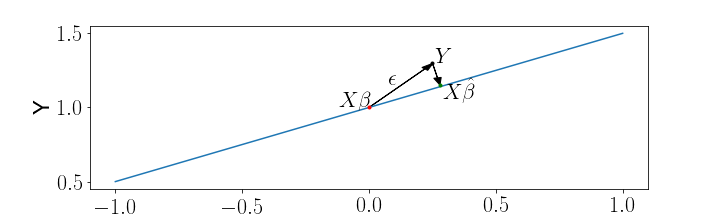
\includegraphics[width=\linewidth]{least_square.png}
  \caption{ Mối liên hệ hình học giữa $X\beta$, $\epsilon$, $Y$ và $X\hat{\beta}$ trong không gian hai chiều. Chú ý rằng $Y-X\hat{\beta}$ vuông góc với $X\hat{\beta} - X\beta$ theo định nghĩa của hình chiếu.}
  \label{fig:boat1}
\end{figure}
Quay trở lại với LSE, để ý rằng ta đã có $X_i\hat{\beta} = X(X^{T}X)^{-1}X^{T}Y_i$, suy ra $X_i\hat{\beta}$ là hình chiếu của $Y_i$ lên một không gian con $S=span(x^{1}, x^{2},...,x^{D})$ và projection matrix $P=X(X^{T}X)^{-1}X^{T}$. Để dễ hình dung hơn thì quan sát Hình 2 để thấy rõ mối quan hệ giữa $Y_i, \epsilon_i, X_i\beta$ và $X_i\hat{\beta}$.\\

Đến đây, ta tiếp tục giả sử $rank(X)=D$ và $\epsilon_1,...\epsilon_n$ là i.i.d, tuân theo phân phối Gaussian với mean 0 và covariance matrix $\sigma^2I_n$, với $\sigma^2$ nào đó. Nói cách khác: 
\[\epsilon \sim N(0, \sigma^2I_n) \]
Ta biết $Y=X\beta + \epsilon$, suy ra:
\[ \hat{\beta} = (X^{T}X)^{-1}X^{T}Y=(X^{T}X)^{-1}X^{T}(X\beta + \epsilon) = (X^{T}X)^{-1}X^{T}X\beta + (X^{T}X)^{-1}X^{T}\epsilon \tag{2}\]
Sử dụng tính chất của phân phối Gaussian sau:
\begin{itemize}

\item Tính chất: Nếu $\epsilon \sim N_d(0, \Sigma)$, thì $B\epsilon \sim N_d(0, B\Sigma B^{T})$ với mọi B thỏa mãn phép nhân $B\epsilon $. (*)

\end{itemize}
Chứng minh tính chất này khá dễ dàng nên mình xin phép được bỏ qua.\\
Quay trở lại với (2):
\begin{itemize}

\item $(X^{T}X)^{-1}X^{T}X\beta= \beta$
\item  Vì $\epsilon \sim N(0, \sigma^2 I_n)$ nên sử dụng tính chất trên của phân phối Gaussian, ta suy ra:  
\[ (X^{T}X)^{-1}X^{T}\epsilon \sim N_d(0, \sigma^2 (X^{T}X)^{-1}X^{T} X (X^{T}X)^{-1}) = N_d(0, \sigma^2 (X^{T}X)^{-1})\]

\end{itemize}
Thay ngược vào (2), ta có: $\hat{\beta} = \beta + N_d(0, \sigma^2 (X^{T}X)^{-1}) \sim N_d(\beta, \sigma^2 (X^{T}X)^{-1}).$
Đến đây ta có một số nhận xét quan trọng sau:
\begin{itemize}

\item $\hat{\beta}$ là một random variable tuân theo phân phối Gaussian với mean là $\beta$ và covariance matrix phụ thuộc vào đại lượng $(X^{T}X)^{-1}$. Miễn là $(X^{T}X)^{-1}$ không quá lớn, ta luôn có một ước lượng xấp xỉ với giá trị đúng.
\item  Least Squared Estmator (LSE) cũng là Maximum Likehood Estimator. Bình thường khi ta nói đến MLE thì ta cần phải có "likelihood" hay nói cách khác là ta cần phải có "density". Thêm nữa, khi làm việc với dữ liệu, muốn có "density" thì ta bắt buộc phải "make assumption" lên data cũng như việc ta đã phải giả sử $\epsilon$ tuân theo phân phối Gaussian thì mới có kết quả này.

\end{itemize}
Chứng minh Least Squared Estmator cũng là Maximum Likehood Estimator (MLE): Như ta giả sử ở trên $\epsilon \sim N_d(0, \sigma^2 I_n)$ và $Y = X\beta + \epsilon$ hay nói cách khác là $Y \sim N_d(X\beta, \sigma^2 I_n)$. Từ đây ta có một statistical model: $(\mathbb{P}_{\beta})_{\beta \in \mathbb{R}^{D}} = {N_d(X\beta, \sigma^2 I_n)}$. Ta có biểu thức density:
\[f(y) = \frac{1}{(\sigma^2 2\pi)^{\frac{1}{2}}}e^{-\frac{||Y-X\beta ||^2_2}{2\sigma^2}} \Longleftrightarrow log(f(y))= -\frac{n}{2}log(\sigma^2 2 \pi) -\frac{1}{2\sigma^2}||Y-X\beta ||^2_2 \]
Suy ra: MLE  $=argmin_{\beta}(||Y-X\beta ||^2_2)=$ LSE.
Ngoài ra, ta cũng suy ra được vài tính chất quan trọng sau:
\begin{itemize}

\item Quadratic risk of $\hat{\beta}$:
\[  \mathbb{E}[|| \hat{\beta} - \beta||^2_2]= \sigma^2 tr((X^{T}X)^{-1}) \tag{3} \]
\item  Prediction error (residual):
\[ \mathbb{E}[||Y-X\hat{\beta}||^2_2] = \sigma^2 (n-D) \tag{4}\]
\item  Unbiased estimator of $\sigma^2$:
\[ \hat{\sigma}^2 = \frac{1}{n-D}||Y-X\hat{\beta}||^2_2 \tag{5}\]

\end{itemize}
Lưu ý rằng ta dễ dàng có quan sát sau: $\hat{\beta} -\beta \sim N_d(0, X^{T}X)^{-1})$\\
Chứng minh (3): ta có $\mathbb{E}[ ||\hat{\beta} - \beta||^2_2]=\sum_{i=1}^{D}\mathbb{E}[(\hat{\beta}_i -\beta_i)^2]=\sum_{i=1}^{D}Var(\hat{\beta}_i)=\sigma^2 tr((X^{T}X)^{-1})$.\\
Trước khi chứng minh (4), ta có vài tính chất sau về projection matrix P lên không gian con $S = span(a_1, a_2,..,a_n)$, và matrix A có các cột là a's:
\begin{itemize}

\item $P^{n}=P$ với mọi số tự nhiên n (6)
\item Eigenvalue của P luôn luôn bằng 0 hoặc bằng 1 (7)
\item  $(I - P)$ cũng là một projection matrix project lên null space của $S^{T}$ (8)

\end{itemize}
Chứng minh (6): Dễ dàng thấy rằng khi ta chiếu 1 điểm lên 1 không gian con nhiều hơn 1 lần, điểm đó sẽ không thay đổi vì nó đã nằm trong không gian con sau lần chiếu đầu tiên, suy ra $P^{n}=P$.\\

Chứng minh (7): Giả sử $\lambda$ là 1 eigenvalue của P cho vector $v$.Sử dụng (6) và theo định nghĩa của eigenvector và eigenvalue, ta có: $\lambda^2v=P^2v= Pv=\lambda v$. Vì $v \neq 0$ nên để thỏa mãn đẳng thức vừa rồi thì $\lambda$ phải bằng 0 hoặc 1.\\

Chứng minh (8): Giả sử $b''$ là hình chiếu của b lên $N(A^{T})$. Dễ dàng nhận thấy rằng vector $b-b'$ phải vuông góc với $C(A)$, suy ra hình chiếu của b lên $N(A^{T})$ cũng chính là $b-b'$, dẫn tới $b''=b-b'=b-Pb=(I-P)b$. Suy ra, $(I-P)$ cũng là một projection matrix.\\

Bây giờ, ta quay lại chứng minh (4), đặt $P'=I-P=I-X(X^{T}X)^{-1}X^{T}$. Ta có:
\[||Y-X\hat{\beta}||^2_2 = ||Y-X(X^{T}X)^{-1}X^{T}Y||_2^2=||(I-X(X^{T}X)^{-1}X^{T})Y||_2^2 = ||P'Y||_2^2 \]
Vì $Y=X\beta + \epsilon$ nên $P'Y=P'X\beta + P'\epsilon$. Để ý rằng $X\beta$ nằm trong column space của $X$, nên khi chiếu $X\beta$ xuống null space của $X$, ta luôn thu được vector 0. Do đó, $P'X\beta = 0$, dẫn tới $P'Y=P'\epsilon$. Từ đây ta có được 
\[\mathbb{E}[||Y-X\hat{\beta}||^2_2]=\mathbb{E}[||P'Y||_2^2]=\mathbb{E}[||P'\epsilon||_2^2] =\mathbb{E}[||P'N(0, \sigma^2 I_n||^2_2)] = \mathbb{E}[||N(0, \sigma^2 P' P')||^2_2] =\mathbb{E}[||N(0, \sigma^2 P')||^2_2]\]
Dấu bằng cuối cùng xảy ra vì $P'$ là một projecttion matrix nên $P'^2=P'$. Chú ý rằng vì $dim(C(X))=D$ nên $dim(N(X^{T}))=n-D$. Đến đây sử dụng cách chứng minh ở (3), ta có $\mathbb{E}[||N(0, \sigma^2 P')||^2_2]=\sigma^2 tr(P')$. Vì $tr(P')=\sum egienvalue$ và eigenvalue của $P'$ chỉ có thể bằng 0 hoặc bằng 1, và số eigenvalue bằng 1 chính bằng $dim(N(X^{T}))=n-D$ nên  $tr(P')=n - D$. Suy ra (4).\\

Dựa vào (4), ta có thể suy trực tiếp ra (5).\\

Ngoài ra, còn 1 định lí về LSE mà mình cho rằng khá khó để chứng minh, như sau:
\begin{itemize}

\item Định lí: $(n-p)\frac{\hat{\sigma}^2}{\sigma^2} \sim \chi^2_{n-D}$ (6)


\end{itemize}
Để chứng minh được (6) ta cần bổ đề sau: Nếu A là một orthogonal matrix thì với X bất kì thỏa mãn phép nhân thì $||UA||_2^{2}=||A||_2^{2}$.\\
Chứng minh bổ đề: $||UA||_2^{2}=(UA)^{T}(UA)=A^{T}U^{T}UA = A^{T}A=||A||_2^{2}$ (vì U là orthogonal matrix).\\

Chứng minh (6): viết lại $(n-p)\frac{\hat{\sigma}^2}{\sigma^2}= \frac{||Y-X\hat{\beta}||^2_2}{\sigma^2} = \frac{||P'\epsilon||^2_2}{\sigma^2}$ (đã đề cập trong khi chứng minh (4)). Viết lại $P' = UDU^{T}$ (decomposition), trong đó U là một orthogonal matrix và D là một ma trận đường chéo trong đó đường chéo chính là các eigenvalue của $P'$ (0 hoặc 1). Từ đó ta có được $||P'\epsilon||^2_2 = ||UDU^{T}\epsilon||^2_2$, vì U là orthogonal matrix nên dựa vào bổ đề trên ta có $||UDU^{T}\epsilon||^2_2=||DU^{T}\epsilon||^2_2$.\\
Vì $\epsilon \sim N_d(0, \sigma^2 I_n)$ nên theo (*) thì $\epsilon'=U^{T}\epsilon \sim N_d(0, \sigma^2UU^{T})=N_d(0, \sigma^2 I_n) \Rightarrow \epsilon = \epsilon'$. Suy ra $||UDU^{T}\epsilon||^2_2=||DU^{T}\epsilon||^2_2=||D\epsilon||^2_2$, dẫn tới $\frac{||P'\epsilon||^2_2}{\sigma^2}=||P'\frac{\epsilon}{\sigma}||^2_2=||P'Z||^2_2=||DZ||_2^2 = \sum_{i=1}^{D}d_{ii} z_i$ với $Z \sim N(0, I_n)$ và $z_i \sim N_d(0, 1)$. Vì $d_{ii}$ là eigenvalue của $P'$ chỉ là 0 hoặc 1 (và số số 1 chính là n -D) nên biểu thức vừa rồi chính là tổng của $n -D$ standard Gaussian, chính là $\chi_{n-D}^2$ (điều phải chứng minh).





\end{enumerate}

\section{Model Selection}
Từ đầu bài viết đến giờ, để có được những kết quả như trên thì ta đã giả sử $Y=X\beta + \epsilon$ với:
\begin{itemize}

\item $Y \in \mathbb{R}^{n}$ là dependent variable, $X\in \mathbb{R}^{nxD}$ là một deterministic matrix.
\item $\beta \in \mathbb{R}^{D}$ là giá trị chưa biết, cần phải ước lượng.
\item $\epsilon \sim N_d{0,\sigma^2 I_n}$

\end{itemize}
Nếu $D$ quá lớn ($D > n$), sẽ có quá nhiều parameters cần được ướng lượng mặc dù sẽ có một vài covariates có thể sẽ chẳng giúp ích gì cho việ ước lượng $\beta$. Tổng quát hơn, quá nhiều covariates gấy ra hiện tượng high variance, hay còn gọi là overfitting. Ngược lại quá ít covariates gây ra hiện tượng high bias, hay còn gọi là underfitting. Một model tốt sẽ đạt đạt được một tỉ lệ cân bằng tốt giữa bias và variance, và model selection giúp ta đi giải quyết vấn đề này.\\

Một model selection sẽ có 2 vấn đề cần được thực hiện:
\begin{itemize}


\item Định nghĩa một score, có thể tưởng tượng là một đại lượng đo độ tốt của model
\item Tìm kiếm trong tất cả các model để tìm model nào có score cao nhất.

\end{itemize}

Cụ thể hơn, ta định nghĩa $S\subset {1,2,..,D}$ và $X_s=\{X_j: j \subset S\}$ là tập con của các covariates. Ta đặt $\beta_S$ là các tọa độ tương ứng với tập các covariates $S$, và $\hat{\beta_S} $ là LSE của $\beta_S$.  Cuối cùng, $X_s$ là một sub-matrix của X bằng cách chỉ giữ lại các chỉ số covariates trong S. Prediction risk được định nghĩa như sau:
\[R(S) = \mathbb{E}\Big[ ||X_S\hat{\beta}_S - Y^{*}||^2_2 \Big ] \]
Trong đó $Y^{*}$ là giá trị của Y trong tương lai (tức là trong tập test set). Mục tiêu của chúng ta là tìm S sao cho giá trị này là nhỏ nhất.\\
Ngoài ra, định nghĩa thêm training error là
\[\hat{R}(S) = ||X_S\hat{\beta}_S - Y ||^2_2 \]
Nếu ta xem $\hat{R}(S)$ là một ước lượng của $R(S)$ thì điều này rất nguy hiểm vì  $\hat{R}(S)$ là một biased estimator của $R(S)$. Chứng minh:
\[ \mathbb{E}\Big [ ||Y^{*} - X_{S}\hat{\beta}_S||_2^2 \Big ] =  \mathbb{E}\Big [ ||Y^{*} -X_{S}\beta_S + X_{S}\beta_S - X_{S}\hat{\beta}_S||_2^2 = \sigma^2 + \mathbb{E}\Big [ ||X_S\beta_S - X_S\hat{\beta}_S||_2^2 \Big ] \Big ] \]
\[ = 2n\sigma^2 + \mathbb{E}\Big [ ||Y - X_S\hat{\beta}_S||_2^2 \Big ] +  2\mathbb{E}[(X_S\beta_s-Y)^{T}(Y - X_S\hat{\beta}_S)] = \mathbb{E}\Big [ ||Y - X_S\hat{\beta}_S ||_2^2 \Big ] + 2tr(Cov(Y,X_S\hat{\beta}_S )) \]
Hay nói cách khác:
\[bias(\hat{R}(S)) = \mathbb{E}[\hat{R}(S)] - R(S) = -2\sum_{i=1}^{n}Cov(Y_i, X_S\hat{\beta}_S) \]
Có thể hình dung về sự bias này là do dữ liệu của chúng ta được sử dụng 2 lần, một lần cho ước lượng $\beta$ và một lần cho ước lược "risk". Khi ta làm việc với data có chiều lớn thì $Cov(Y_i, X_S\hat{\beta}_S)$ sẽ lớn dẫn tới độn chính xác sẽ giảm đi nhiều. Chính vì vậy người ta đã nghĩ ra các phương pháp khác để ước lượng độ risk của model như sau.
\begin{enumerate}
\item Mallow's $C_p$ statistic\\
Mallow's $C_p$ statistic được định nghĩa như sau 
\[\hat{R}(S) = \hat{R}(S) + 2|S|\hat{\sigma}^2 \tag{9} \]
Trong đó $|S|$ là "the number of terms" trong S và $\hat{\sigma}^2$ là ước lượng của $\sigma^2$ (lưu ý $\sigma^2$ ở đây là trong dạng full covariates). Điều này dễ có thể suy ra thì việc muốn giảm bias thì chỉ cần đơn giản cộng training error và bias. Đại lương đầu tiên ở (9) đo đọ tốt của model (fit of model) ở training set, đại lượng thứ hai đo đọ phức tạp của model. Cuối cùng ta có thể hiểu để tìm một model tốt sẽ nảy sinh ra một sự đánh đổi giữa độ fit và độ phức tạp.
\item BIC (Bayesian information criterion)\\
Với BIC, ta chọn model sao cho biểu thức sau đạt giá trị lớn nhất
\[BIC(S) = l_s -\frac{|S|}{2}log(n) \]
BIC có một cái giải thích theo hướng Bayesian. Giả sử $S = \{S_1,..,S_m \}$ là tập hợp các model, thêm rằng ta gasn prior $\mathbb{P}(S_j) = \frac{1}{m}$ trên tất cả các model. Từ đó có thể chỉ ra được rằng xác suất posterior cho một model có thể được xấp xỉ như sau:
\[ \mathbb{P}[S_j|data] \approx \frac{e^{BIC(S_j)}}{\sum_{i=1}^{m}e^{BIC(S_i)}}\] 
Nhìn vào biểu thức trên ta có thể thấy chọn một model có BIC lớn nhất tương đương chọn một model với xác suất posterior cao nhất. Sâu hơn ta có thể thấy BIC cũng giống như Mallow's $C_p$, nhưng ở BIC ta đánh mạnh tay hơn vào độ phức tạp của model (có thể hiểu ta trừng phạt mạnh hơn), dẫn tới việc ta sẽ có xu hướng chọn một model đơn giản hơn phương pháp Mallow's $C_p$ (trong trường hợp độ tốt là như nhau).
\end{enumerate}
Một điều dễ dàng suy ra với mỗi tiêu chí trên là tương đương với việc tìm $\hat{\beta} \in \mathbb{R}^{D}$ sao cho biểu thức sau đạt giá trị nhỏ nhất
\[ ||Y-X\beta||^2_2 + \lambda ||\beta||_0 \]
Trong đó $||\beta||_0$ là số số khác 0 trong vector $\beta$. Đây là một vấn đề khó vì ta không thể đơn giản đạo hàm rồi tìm ra $\hat{\beta}$ vì đây không phải là một hàm lồi, và để tìm ra  $\hat{\beta}$ ta phải tìm trong tất cả các trường hợp $S \subset \{1,..,D \}$ ($2^{D}$ estimators). Chính vì thế người ta đã thay thế $||\beta||_0$ bằng p-norm ($p \geq 1$) của $\beta$. Bằng cách thay thế như vậy, hàm $f(\beta) = ||Y-X\beta||^2_2 + \lambda ||\beta||_p$ trở thành hàm lồi. p=1 và p=2 là các giá trị mình thường thấy hay được sử dụng trong Linear Rgression.
\begin{figure}
  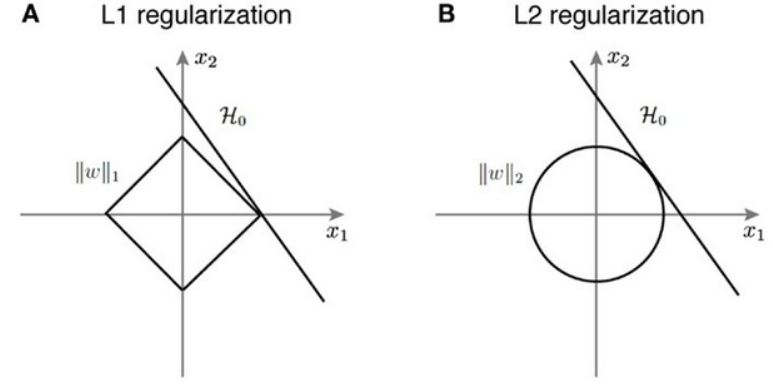
\includegraphics[width=\linewidth]{lasso.png}
  \caption{So sánh L1 và L2. Nguồn: quora.com}
  \label{fig:boat1}
\end{figure}
\begin{itemize}

\item p=1 hay còn được gọi là Lasso. Lưu ý nếu p=1 thì $f(\beta)$ là hàm convex nhưng nó không có đạo hàm tại điểm 0 (dễ thấy vì hàm giá trị tuyệt đối không có đạo hàm tại 0). Lasso có một tính chất thú vị là nó sẽ "shrink" các covariates ít quan trọng. Chính vì thế khi làm việc với dữ liệu nhiều chiều, người ta hay sử dụng Lasso để loại bỏ đi những feature không quan trọng. Để thấy điều này, chú ý rằng để $f(\beta) = ||Y-X\beta||^2_2 + \lambda ||\beta||_1$ đạt nhỏ nhất tương đương với việc để $||Y-X\beta||^2_2$ đạt nhỏ nhất và phải thỏa mãn thêm điều kiện sau.
\[\sum_{i=1}^{D}|\beta_i| \leq \gamma\]
Trong đó $\gamma$ là một giá trị phù hợp (phương pháp Lagrance). Khi đó, quan sát Hình 3, giả sử đường thẳng $H_0$ là các giá trị của $||Y-X\beta||^2_2$ và hình vuông và hình tròn lần lượt là đồ thị của $||w||_1 \leq \gamma$ và của $||w||_2 \leq \gamma$. Khi đó, với L2 thì giao điểm của $H_0$ và $||w||_2$ đều có thành của $x_1, x_2$ khác 0. Ở phía bên kia thì vì tính chất đặc biệt của đồ thị  $||w||_1 \leq \gamma$, giao điểm của $H_0$ có thành phần $x_2=0$. Có nghĩa là với L1 thì nó đã loại trừ vai trò của $x_2$ trong việc tìm giá trị nhỏ nhất của $f(\beta)$.




\end{itemize}


\begin{thebibliography}{9}
\bibitem{latexcompanion} 
All of statistic. 
\textit{}
Larry Wasserman, 2003.
\bibitem{latexcompanion} 
Statistic for application (lecture slide). 
\textit{}
Philippe Rigollet, 2016.

\bibitem{latexcompanion} 
The Truth about Linear Regression (CMU statistics). 
\textit{}
Cosma Rohilla Shalizi.

\bibitem{latexcompanion} 
Pattern Recognition and Machine Learning. 
\textit{}
Christopher M. Bishop.

\end{thebibliography}


\end{document}